\documentclass{paris17}
\usepackage{amsmath}
\usepackage{graphicx}
\usepackage{graphicx}
\usepackage{caption}
\usepackage{subcaption}
\usepackage{floatrow}
% Table float box with bottom caption, box width adjusted to content
\newfloatcommand{capbtabbox}{table}[][\FBwidth]
\usepackage{capt-of}% or \usepackage{caption}
\usepackage{booktabs}
\usepackage{varwidth}


\begin{document}

\section{Introduction}

Imaging and velocity analysis are the most computationally intensive parts of seismic processing. As a results researchers are always trying to find ways to speedup these processes \cite[]{bednar,Stork}.  One approach used to speed up downward continuation based algorithms is to recognize that the earth attenuates seismic signals.  As a result, as we push the wave-field down in depth, we can ignore higher and higher frequencies and still obtain an accurate image\cite[]{Clapp.sep.111.bob3}.  This approach lowers the cost as you increase in depth. This technique is well suited for downward continuation based approaches which are done frequency by frequency.  Reducing the frequencies downward continued as a function of depth  is particularly effective in combination with recognizing that there was no reason to propagate waves a large distance from the source at early times.  While following the wavefield is used routinely in RTM,  taking advantage of attenuation is not commonly used.  Reasons include: the cost of propagation with an attenuated wave equation, attenuation is a function of medium parameter, and propagation is generally done in the the time, rather frequency domain.

In this paper I use a constant-Q approximation based on the work of \cite[]{zhu}.  As I propagate my source I resample my medium based on the maximum frequency that has not been significantly attenuated. Combining this approach with following the wave-field, I show that I can achieve significant computational speedups.

\section{Method and Theory}

\subsection{Modeling}

Explicit finite difference modeling is constrained by figuring  out a sampling in time and space that results in stable propagation and does not create dispersive events.  For stability the Courant-Friedrichs-Lewy condition \cite[]{courant1967partial} must be met.  Stability is a function of limiting what percentage of a grid cell energy can move in one time step. Stability is therefore a function of the maximum velocity $v_{max}$, the minimum spatial sampling $d_{min}$, and the time step $dt$. For stability, we have $v_{max}\frac{dt}{d_{min}} < .5$.  The stability condition pushes one to use larger spatial sampling (faster, but less resolution) and/or finer time sampling (more expensive).  Dispersion, on the other hand, is a function of the minimum velocity $v_{min}$, the maximum frequency $f_{max}$, and the maximum spaital sampling $d_{max}$.   To avoid grid dispersion we need to  sample a given frequency with a minimum number of points.  There isn't a consensus on the minimum number
of points. For the purpose of this paper I will require  3.2  points therefore, we have $\frac{v_{min} }{f_{max}d_{max}} > 3.2 \label{eq:dispersion}$.

The dispersion constraint pushes us towards smaller (more expensive) spatial sampling, because of the stability constraint, and results in smaller the steps.  Minimizing dispersion is the real reason for the expense of finite differences.  To avoid grid dispersion and achieve the same level of stability the number of operations increase by the fourth power (three due to space sampling and one for time).

From observation we know that the earth attenuates acoustic signals.  Attenuation varies as a function of frequency and earth materials. The first approximation I am going to use is the concept of the constant Q model introduced by \cite{Kjartansson.sep.23}.  Q is defined as $Q=2 \pi \left( \frac{E}{\partial E}\right)$, where $\frac{E}{\partial E}$ is the fraction of energy lost per cycle. The larger the $Q$ value, the less energy loss per cycles.  The constant Q assumption assumes that energy dies out is a function of the number of wavelengths traveled through a medium. The higher the frequency, the faster the energy is attenuated.

\subsection{Constant Q formulation}

Our theory is built on the foundation of \cite[]{zhu2014theory}. It is a time-domain differential equation for modeling seismic wave propagation in constant-Q viscoelastic media based on fractional spatial derivatives, specifically Laplacian differential operators of fractional order.  The stress–strain relation is derived from the classical equation expressed in terms of fractional time derivatives. The formulation has the advantage of not requiring additional field variables that increase the computer time and storage significantly \cite[]{zhu2014theory}.

We first extend the formulation of \cite[]{zhu2014theory} from the 2D viscoelastic case to the 3D viscoelastic case. Note that the Laplacian differential operators of fractional order bring extra computational costs to the elastic modeling, we approximate it with the conventional Laplacian operators, which significantly reduces the computing complexities. Also, we further reduce the computational costs by ignoring the dispersion terms because it make little effects compared to the attenuation of the signals. As a result, our equations are then

\begin{equation}
\begin{bmatrix} \sigma_{11}\\ \sigma_{22}\\ \sigma_{33} \end{bmatrix} = \begin{bmatrix} \frac{\partial \tau_p^{(1)}}{\partial t} + c_{11} & \frac{\partial \tau_p^{(1)}}{\partial t} - 2\frac{\partial \tau_s^{(1)}}{\partial t} +c_{12}& \frac{\partial \tau_p^{(1)}}{\partial t} - 2\frac{\partial \tau_s^{(1)}}{\partial t} +c_{13} \\ \frac{\partial \tau_p^{(2)}}{\partial t} - 2\frac{\partial \tau_s^{(2)}}{\partial t} +c_{12}& \frac{\partial \tau_p^{(2)}}{\partial t} + c_{22} & \frac{\partial \tau_p^{(2)}}{\partial t} - 2\frac{\partial \tau_s^{(2)}}{\partial t} +c_{23}\\ \frac{\partial \tau_p^{(3)}}{\partial t} - 2\frac{\partial \tau_s^{(3)}}{\partial t} +c_{13} & \frac{\partial \tau_p^{(3)}}{\partial t} - 2\frac{\partial \tau_s^{(3)}}{\partial t} +c_{23} & \frac{\partial \tau_p^{(3)}}{\partial t} + c_{33} \end{bmatrix} \begin{bmatrix} \epsilon_{11}\\ \epsilon_{22}\\ \epsilon_{33} \end{bmatrix}
\end{equation}

\begin{equation}
  \sigma_{12} = \left ( 2\frac{\partial}{\partial t} \left( \frac{c_{11}-c_{12}}{2}c_s^{(2\gamma_s-1)}\sin(\pi\gamma_s) \right) + c_{66} \right )\times \epsilon_{12}
\end{equation}

\begin{equation}
  \sigma_{13} = \left ( 2\frac{\partial}{\partial t} \left( \frac{c_{33}-c_{13}}{2}c_s^{(2\gamma_s-1)}\sin(\pi\gamma_s) \right) + c_{55} \right )\times \epsilon_{13}
\end{equation}

\begin{equation}
  \sigma_{23} = \left ( 2\frac{\partial}{\partial t} \left( \frac{c_{22}-c_{23}}{2}c_s^{(2\gamma_s-1)}\sin(\pi\gamma_s) \right) + c_{44} \right )\times \epsilon_{23}
\end{equation}

\begin{equation}
  \tau_p^{(1)} = c_{11}C_p^{2\gamma_p - 1}\sin(\pi \gamma_p)
\end{equation}

\begin{equation}
  \tau_s^{(1)} = \frac{c_{11} - c_{13}}{2}C_s^{2\gamma_s - 1}\sin(\pi \gamma_s)
\end{equation}

\begin{equation}
  \gamma_{p,s}=\frac{1}{\pi}\tan^{-1}(\frac{1}{Q_{p,s}})
\end{equation}

where $\sigma$ is the stress tensor; $\epsilon$ is the strain tensor; $c_{ij}$ is the forth-order stiffness tensor; $C_p$ and $C_s$ are the velocities of P-wave and S-wave. $Q_{p,s}$ is the constant factor for the attenuation of P-wave and S-wave respectively. Note that we only present how $\tau_p^{(1)}$ and $\tau_s^{(1)}$ are derived, $\tau_p^{(2)}$,$\tau_p^{(3)}$, $\tau_s^{(2)}$ and $\tau_s^{(3)}$ can be derived in a similar way.

Our constant Q formulation is relatively computationally economic because we preserve the original workflow of elastic modeling while adding a few terms in the calculation of stress tensors from train tensors.

\subsection{GPU optimizations}

The reason why GPUs outperforms CPUs significantly on many scenarios is that the architecture of GPUs favors throughput of many data-parallel tasks over the latency of a single thread. We have an efficient parallel design on the GPU platform with three main strategies.

Firstly, we fully utilize the different hierarchical memory of the GPU. We keep a set of constant variables such as the derivative coefficients in the constant memory and the read-only cache. As the 64KB first-level cache can be configured as different combinations between L1 cache and shared memory, we configure it dynamically based on different computing scenarios. For the stencil computation, we configure the first-level cache by setting the sizes of shared memory and L1 cache to be 48 KB and 16 KB, respectively, which achieves a high computation performance based on P. Micikevicius’ 3D stencil design. For others, we prefer to configure the first-level cache as L1 cache if we don't use shared memory explicitly.

Secondly, we carefully tune the number of registers per thread to maximize the occupancy of GPUs. Since the access pattern of GPU global memory in the stencil kernel is irregular, the more threads are busy, the less latencies it is for memory access. However, as the number of registers is limited in a streaming multiprocessor (SM), increasing the number of registers per threads will decrease the number of active warps. So it is important to have a strategy to balance them. We first remove the intermediate variables to reduce the number of registers per threads. Then we dynamically tracking the performance by adjusting the block size and the \emph{maxrregcount} compiler option.

Thirdly, we design a computation and communication overlapping scheme to maximize the concurrency of different resources. The entire wavefield domain is divided into 4 subdomain, each assigning to a GPU shown in Figure \ref{fig:domain-decomposition}. Note that we need ghost cells to store and exchanges the halos, denoted by the arrows. In each subdomain, we further divide it into three parts, the halo part, the outer part and the inner part shown in Figure \ref{fig:task-decomposition}. The computation of inner and outer parts are assigned to different CUDA streams so that they are executed concurrently. When the computation of the outer part is finished, the GPU starts exchanging halos with its neighbors. In this way, the computation of the inner part can hide the communication shown in Figure \ref{fig:overlap}.

\begin{figure}[h]
    \centering
    \begin{subfigure}[b]{0.3\textwidth}
        \centering
        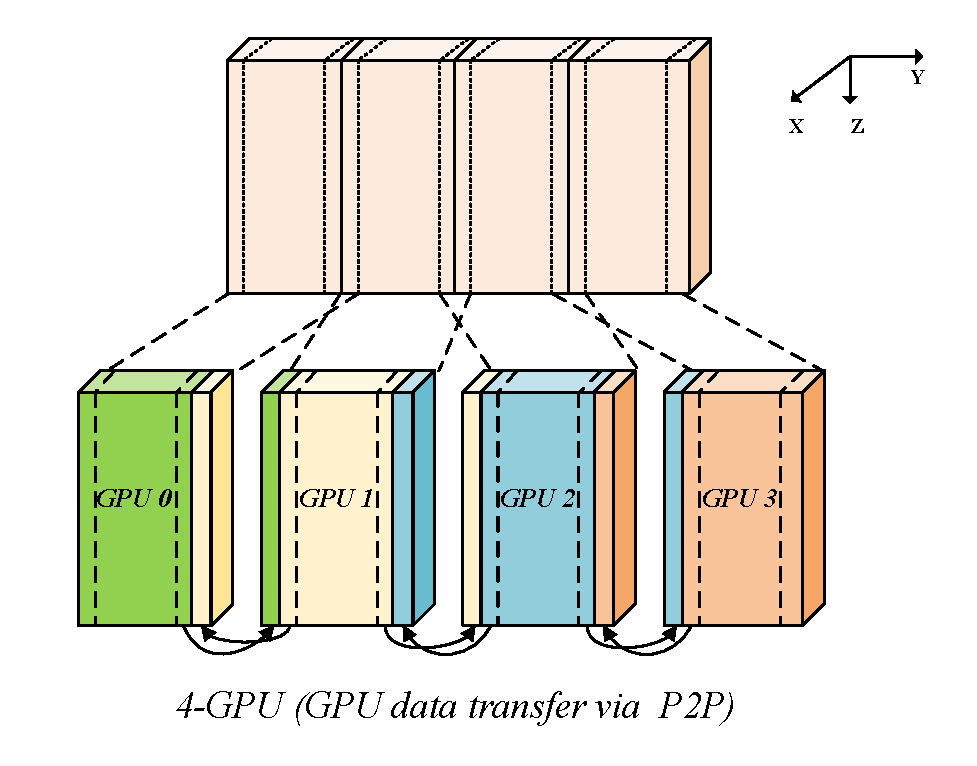
\includegraphics[height=1.3in]{./fig/domain-decompose.pdf}
        \caption{Domain decomposition}
        \label{fig:domain-decomposition}
    \end{subfigure}%
    ~
    \begin{subfigure}[b]{0.3\textwidth}
        \centering
        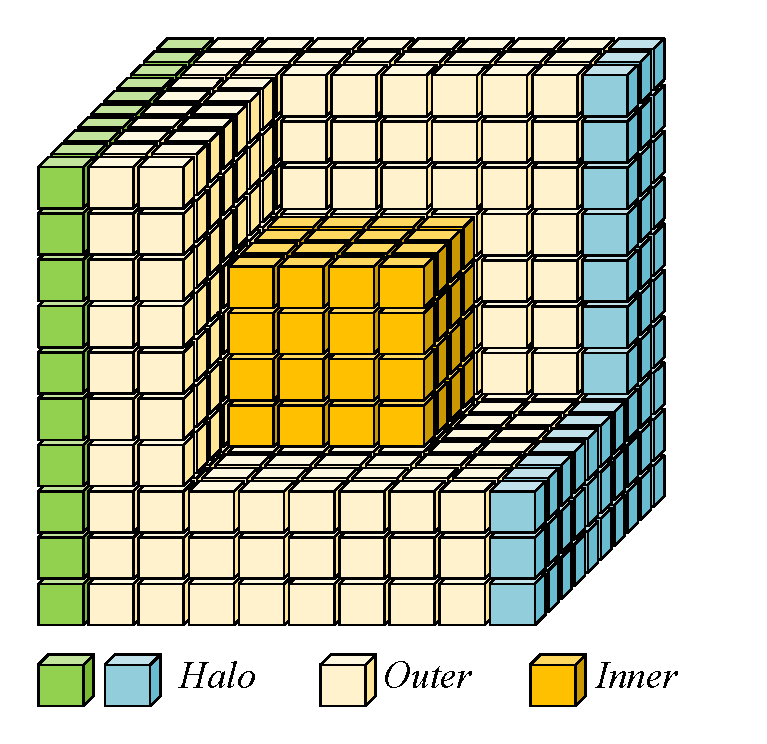
\includegraphics[height=1.3in]{./fig/inner-outer.pdf}
        \caption{Task decomposition}
        \label{fig:task-decomposition}
    \end{subfigure}
    ~
    \begin{subfigure}[b]{0.3\textwidth}
        \centering
        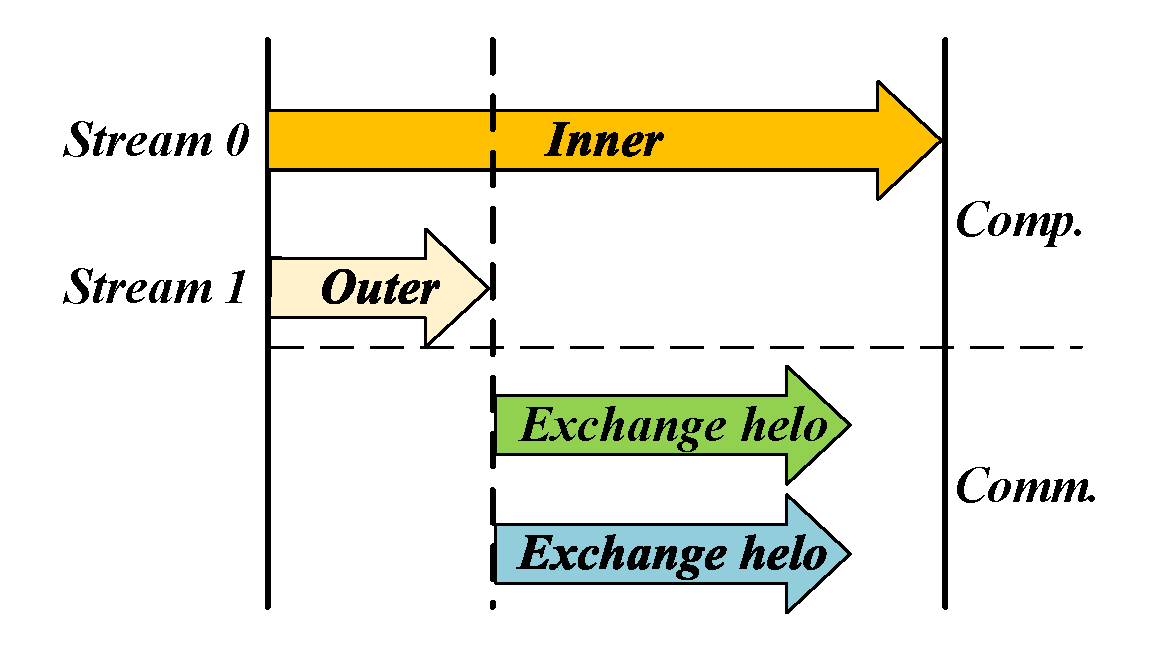
\includegraphics[height=1.1in]{./fig/overlap.pdf}
        \caption{Comp. \& Comm. overlapping}
        \label{fig:overlap}
    \end{subfigure}
    \caption{Computation and communication overlapping over multiple GPUs.}
\end{figure}

\section{Experiments}

Figure xxx shows the wave-field using the standard acoustic wave equation (left) and an attenuation wave-field (right). Note the difference in the frequency content. This is can be more clearly seen in Figure xxx which shows the spectrum of wave-field at 0.9 seconds with $Q_p = Q_s = 20$.

Notice the energy decay of frequency over time. The key observation is that there is no reason to worry about dispersion at frequencies that have attenuated. Specifically, I redo my dispersion calculation (equation 2) several times while propagating a wave-field. At each time block I use a fmax based on frequencies whose energy has not been reduced more than some percentage (in this paper 96\%). As a result, as I forward propagate in time my grid cells, and if I desire, time sampling, get larger. Figure 3 shows the speedup factor (defined as the number of grid cells times time steps) as a function of propagation time for different Q values. The longer the time record, the more using Q pays off in terms speed up. Using this approach the early time steps dominate the computation. For example assuming an initial maximum frequency of 90Hz and a constant velocity of 2000m/s, a Q value of 200, the total speedup is 4 even though most of the propagation time shows significantly more speedup. Figure 4 shows the speedups for Q values ranging from 150 to 350.

\begin{figure}[h]
    \centering
    \begin{subfigure}[b]{0.3\textwidth}
        \centering
        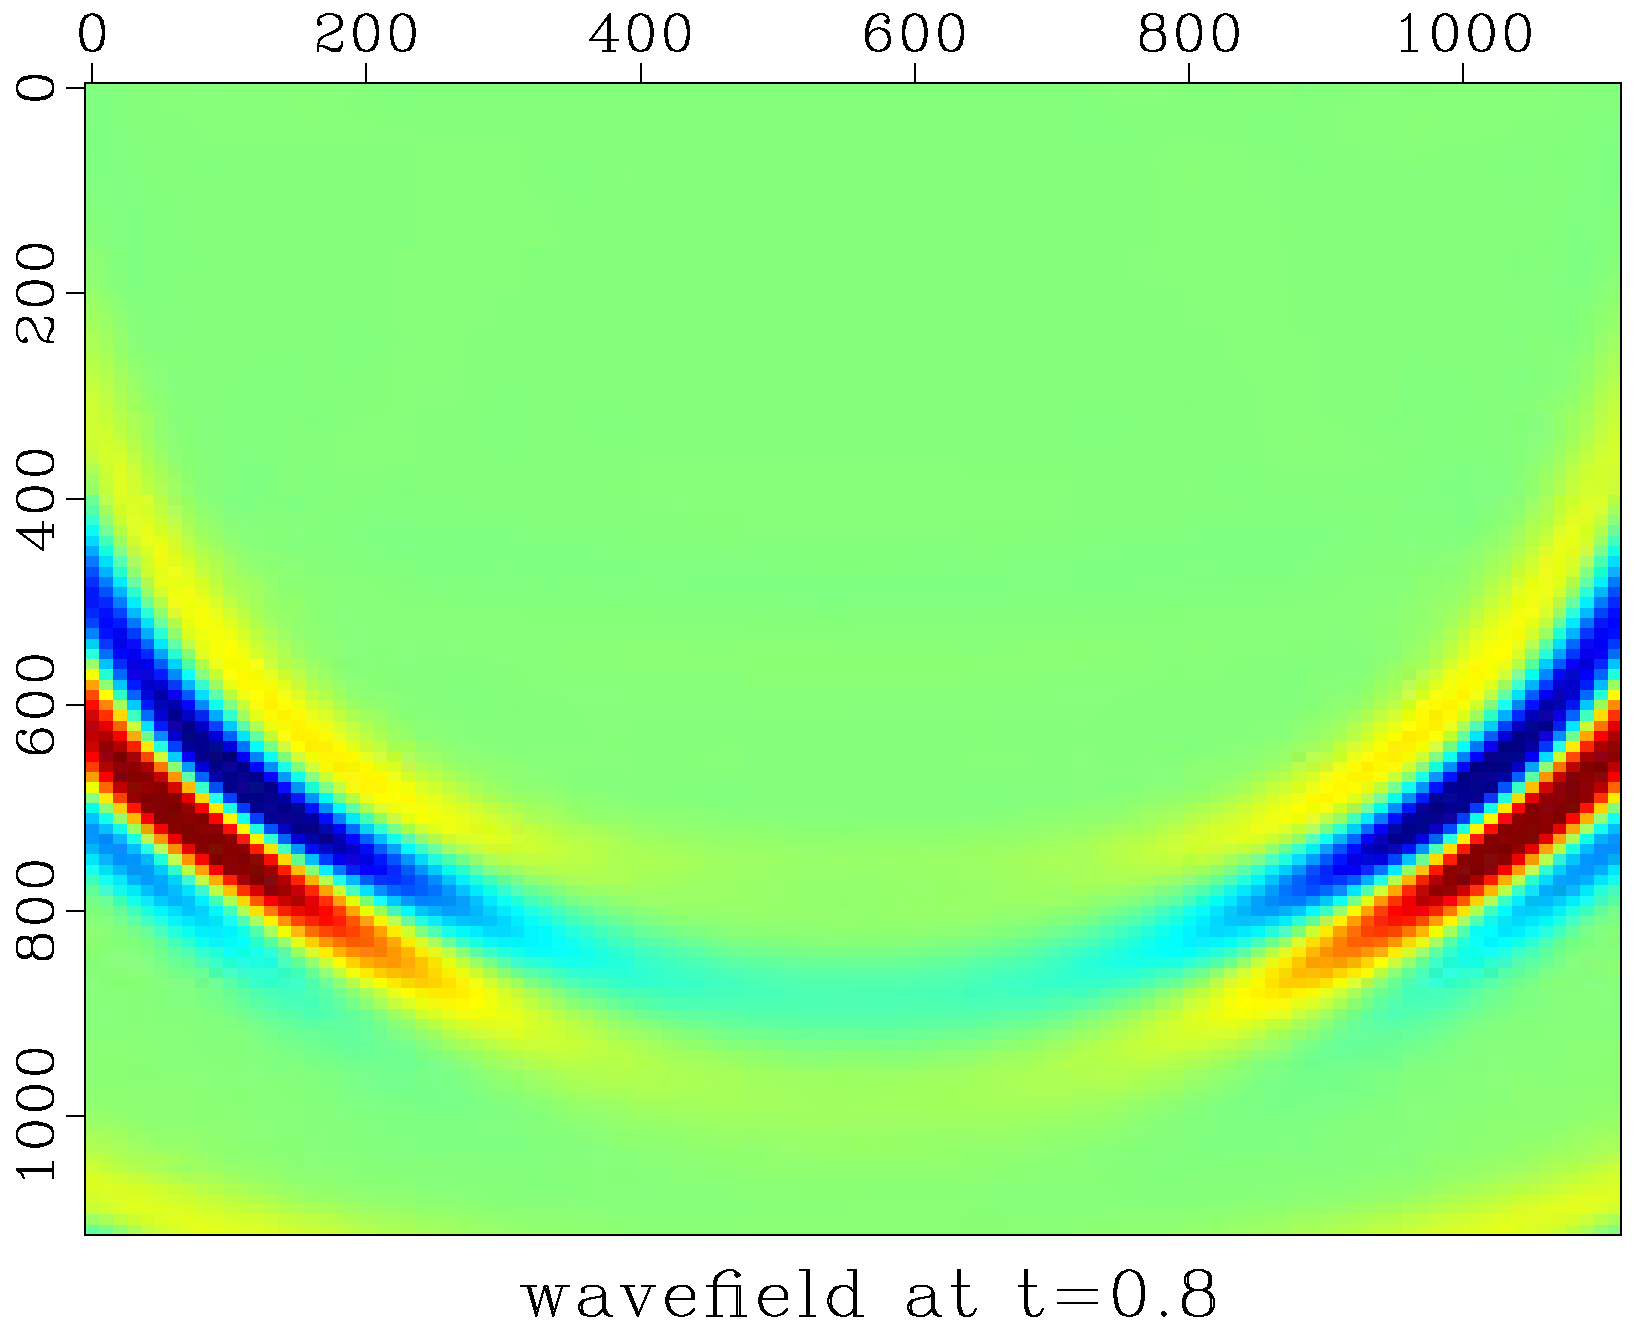
\includegraphics[height=1.3in]{./fig/std.pdf}
        \caption{Wavefield without attenuation}
    \end{subfigure}%
    ~
    \begin{subfigure}[b]{0.3\textwidth}
        \centering
        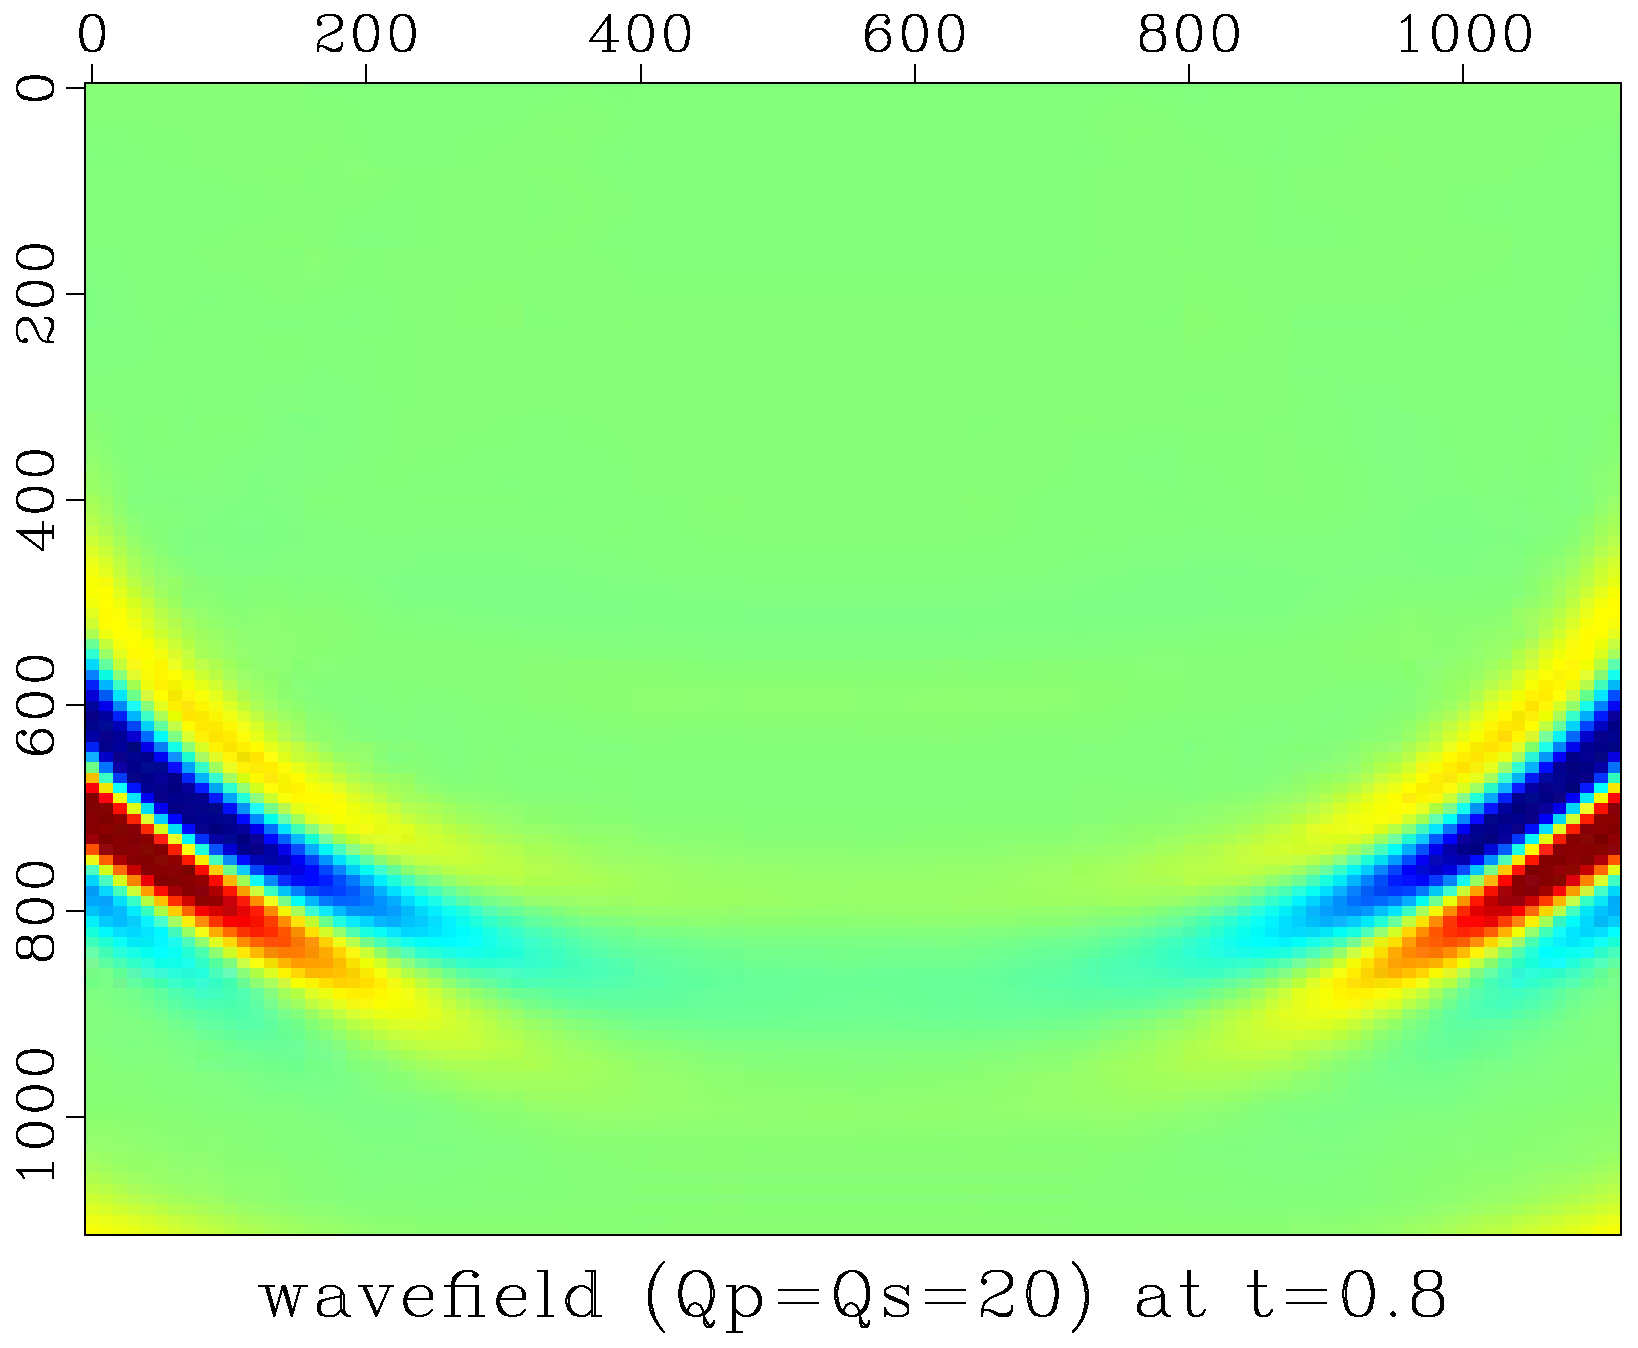
\includegraphics[height=1.3in]{./fig/q20.pdf}
        \caption{Wavefield with attenuation}
    \end{subfigure}
    ~
    \begin{subfigure}[b]{0.3\textwidth}
        \centering
        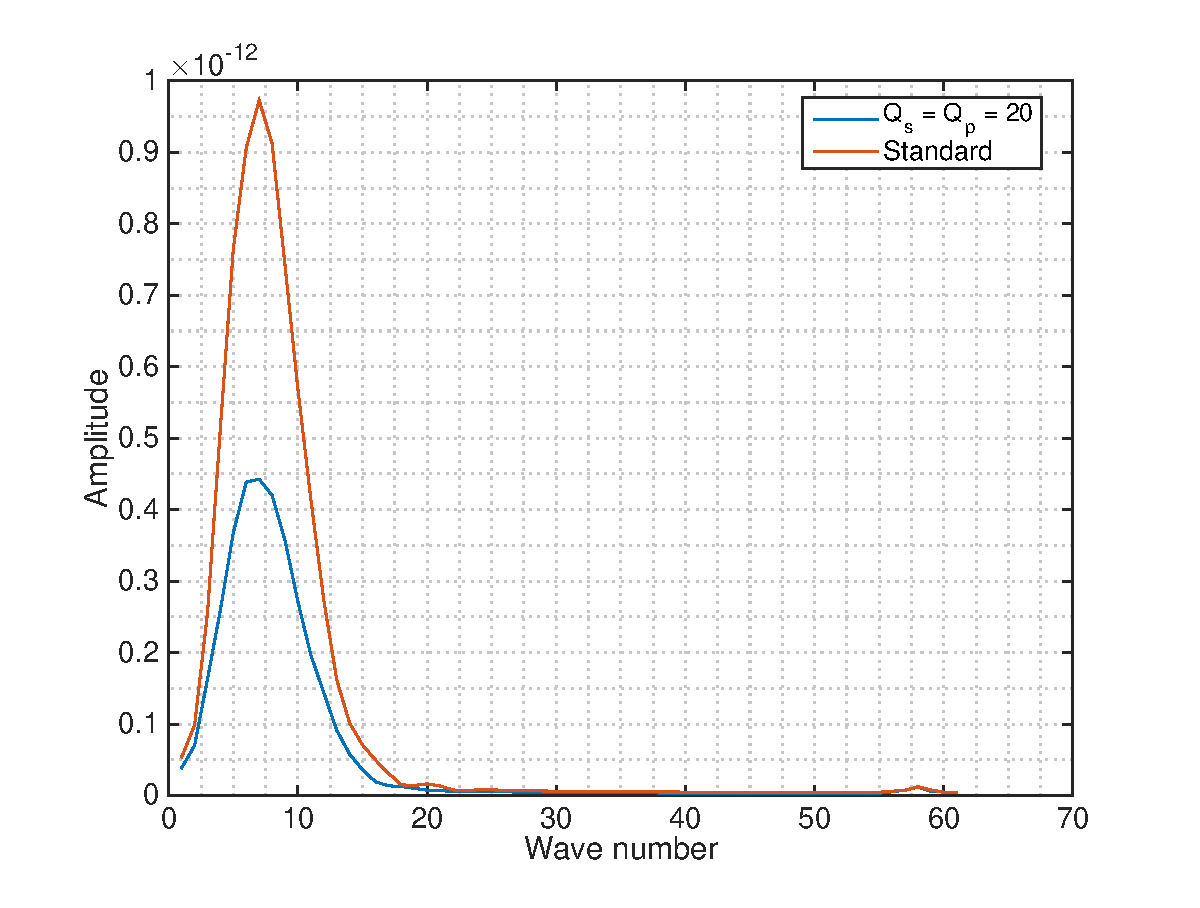
\includegraphics[height=1.3in]{./fig/spec.eps}
        \caption{Spectrum of the wavefields}
    \end{subfigure}
    \caption{Wavefields with and without attenuation.}
\end{figure}

Another speedup trick used by many when doing modeling/migration is to recognize that there is no need to propagate the wave-fields significantly away from the source at early times. The number of cells we need to propagate increases as a power of three (expanding wave-field) in modeling, and somewhat less in migration due to the spatial extent of our receivers. This speedup trick is most effective at early times and useless at late times when energy has propagated throughout the model, the opposite behavior as the constant-Q trick. Combining the two tricks is where we begin to see big payoffs. The left plot of Figure 6 shows the result of combining the two approaches for different values of Q.

Table xxx shows the performance speedup on using different number of GPUs. Through combining the GPU optimization schemes above, the GPU design amoung four K40 cards improve the performance by upto xxx times over xxx cores. Note that the CPU design is also tuned by using multi-threading and vectorizations.
\begin{figure}[h]
    \centering
    \begin{subfigure}[b]{0.4\textwidth}
        \centering
        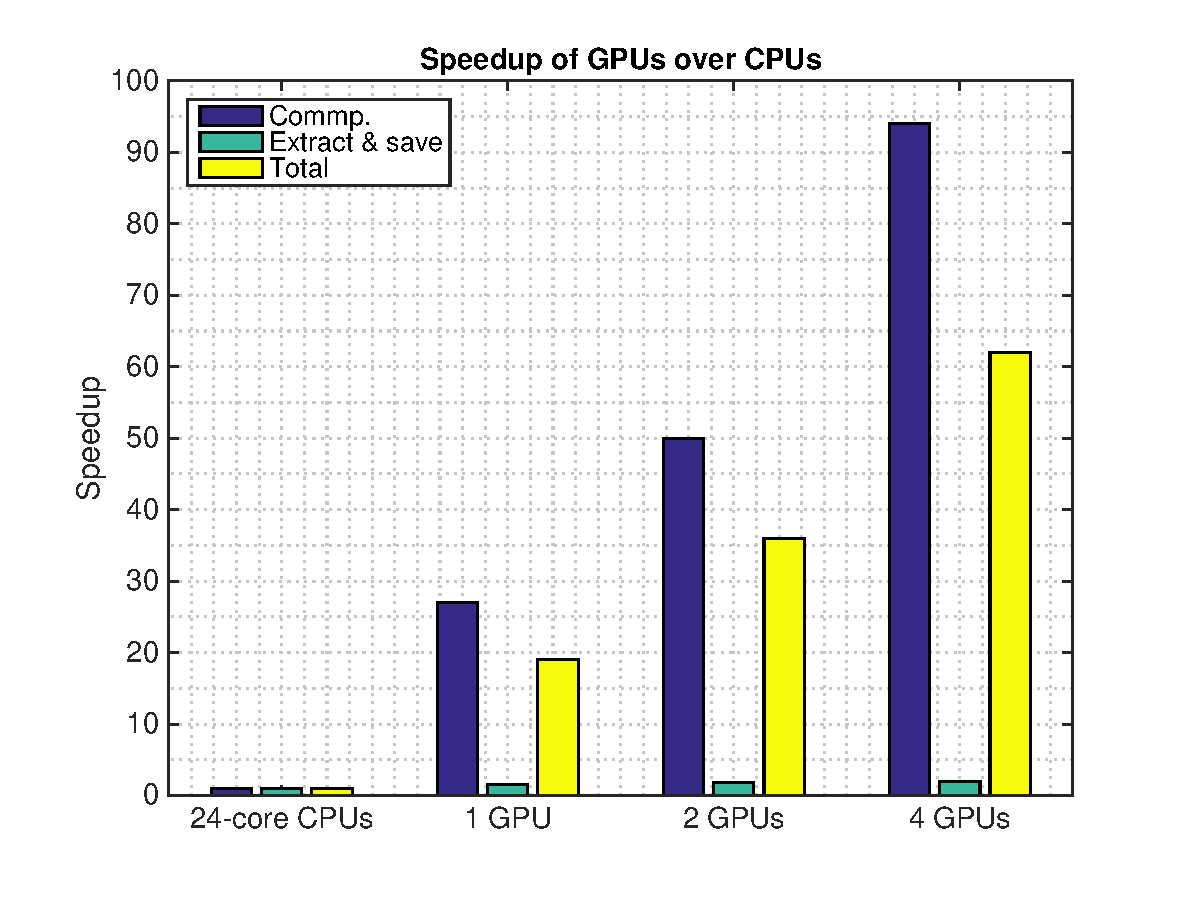
\includegraphics[height=1.5in]{./fig/speedup.eps}
%        \caption{Wavefield without attenuation}
    \end{subfigure}%
    ~
    \begin{subfigure}[b]{0.4\textwidth}
        \centering
        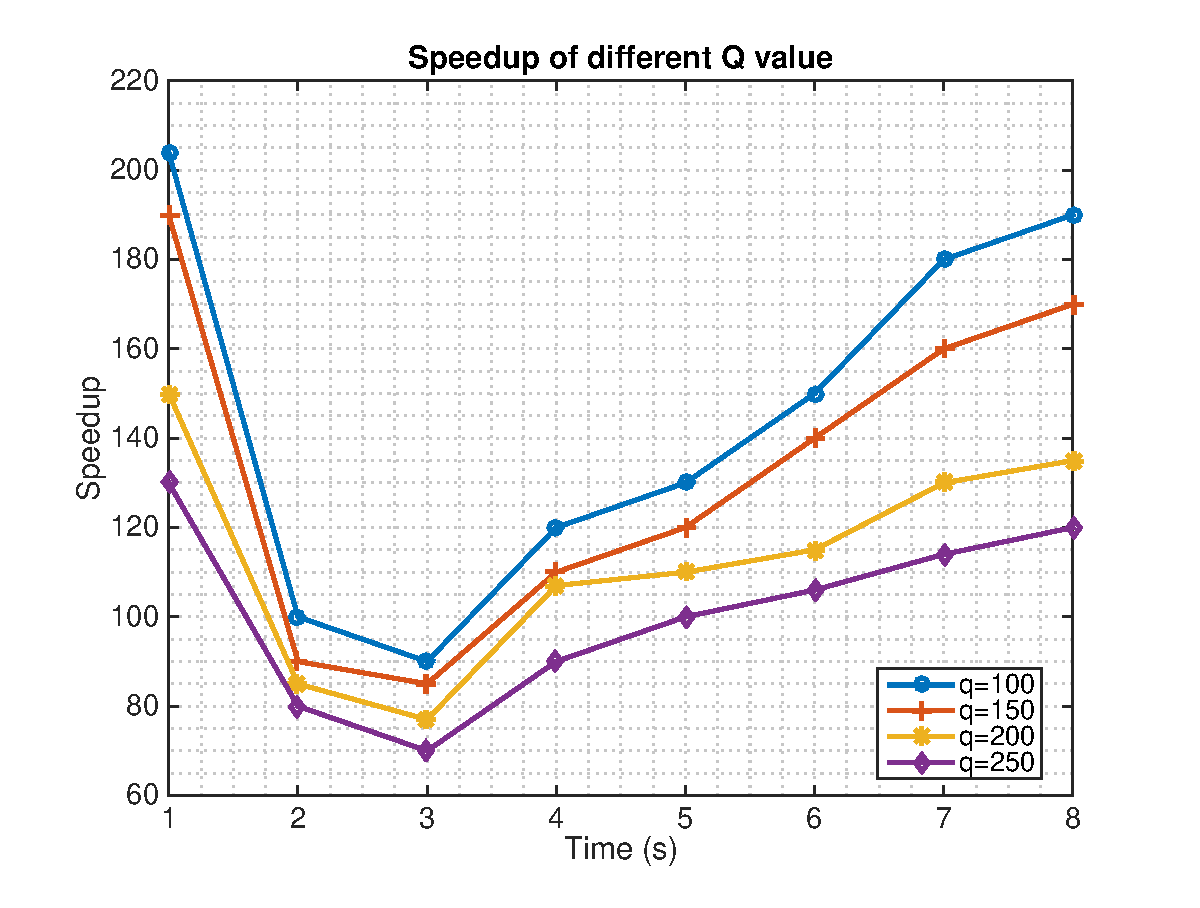
\includegraphics[height=1.5in]{./fig/speedup_q.eps}
%        \caption{Wavefield with attenuation}
    \end{subfigure}
    \caption{Wavefields with and without attenuation.}
\end{figure}


The memory optimizations achieve the best usage of the hierarchical GPU spaces, while tuning the register usage per thread reaches a tradeoff to maximize the computing efficiency. Furthermore, the halo updating is largely hidden within the computations. So we achieve an inspiring performance speedup.

\section{Conclusions}

This is the first sentence of the conclusions.


\bibliography{bob}


\end{document}

